\section{The Density Operator}
So far: State vector $\statepsi$ describing a quantum state.
Convenient alternative formulation for quantum systems about which we 
only have partial information: \\
\underline{Density operator} (also called density matrix)

\subsection{Ensembles of quantum states}
Consider a quantum system which is in one of several states $\ket{\psi_i}$
with probability $p_i$: \underline{Ensemble} of quantum states
$\{p_i, \ket{\psi_i} \}$ \\
The \underline{density operator} $\rho$ of the ensemble $\{p_i, \ket{\psi_i} \}$
is defined as 

\begin{equation}
    \rho = \sum_i p_i \ket{\psi_i} \bra{\psi_i}
\end{equation}

Quantum mechanics in terms of the density operators:
\begin{itemize}
    \item Unitary operation: a unitary transformation $U$ maps each
    $\ket{\psi_i} \mapsto U \ket{\psi_i}$, and the ensemble to  $\{p_i, U \ket{\psi_i} \}$.
    Thus the density operator is transformed as 
    \begin{equation}
        \rho \stackrel{U}{\mapsto} \sum_i p_i U \ket{\psi_i} 
            \underbrace{\bra{\psi_i} U^\dag}_{(U\ket{\psi_i})^\dag} 
        = U \underbrace{(\sum_i p_i \ket{\psi_i} \bra{\psi_i})}_{\rho} U^\dag 
        = U \rho U^\dag
    \end{equation}

    \item Measurements: measurement operators $\{M_m\}$, if the system is in state
    $\ket{\psi_i}$, then the probability for result $m$, given $i$, is 
    \begin{equation}
        p(m|i) = \braketmatrix{\psi_i}{M_m^\dag M_m}{\psi_i} = 
            tr \left[ M_m^\dag M_m \ket{\psi_i} \bra{\psi_i} \right]
    \end{equation}
    Thus overall probability for result m is:
    \begin{align}
        p(m) &= \sum_i p(m|i) p_i = 
            \sum_i tr \left[ M_m^\dag M_m \ket{\psi_i} \bra{\psi_i} \right] p_i \\
            &= tr [ M_m^\dag M_m \underbrace{\sum_i p_i \ket{\psi_i} \bra{\psi_i}}_{\rho}] 
            = tr [M_m^\dag M_m \rho]
    \end{align}

    Density operator $\rho_m$ after obtaining measurement result $m$? \\
    State $i$ collapses to 
    \begin{equation}
    \ket{\psi_i} \mapsto \frac{M_m \ket{\psi_i}}{|| M_m \ket{\psi_i}||} =: \ket{\psi_i^m}
    \end{equation}
    Thus:
    
    \begin{align}
        \rho_m &= \sum_i p(i|m) \ket{\psi_i^m} \bra{\psi_i^m} 
            = \sum_i p(i|m) \frac{M_m \ket{\psi_i} \bra{\psi_i^m} M_m^\dag}
            {\underbrace{|| M_m \ket{\psi_i}||^2}_{p(m|i)}} \\
            &\stackrel{\text{Bayes Theorem}}{=} \sum_i p_i \frac{M_m \ket{\psi_i} \bra{\psi_i} M_m}{p(m)}
            = \frac{M_m \rho M_m^\dag}{tr[M_m^\dag M_m \rho]}
    \end{align}

    Note that $\rho_m$ is now expressed in terms of $\rho$ and the measurement
    operators, without explicit reference to the ensemble $\{p_i, \ket{\psi_i} \}$.
\end{itemize}

\subsection{General properties of the density operator}

Characterization of density operators: An operator $\rho$ is the
density matrix associated to some ensemble $\{p_i, \ket{\psi_i} \}$ if and only if:
\begin{enumerate}
    \item $tr[\rho] = 1$ (\textit{trace condition})
    \item $\rho$ is a positive operator (\textit{positivity condition})
\end{enumerate}
Remark: $\rho$ is called a \underline{positive operator} if it is Hermitian and all its
eigenvalues are non-negative, equivalent 
$\braketmatrix{\varphi}{\rho}{\varphi} \geq 0$ for all vectors $\ket{\varphi}$. 

Proof is in the official lecture notes on Moodle. \\

From now on, we define a density operator as positive operator $\rho$ with
$tr[\rho] = 1$. \\
Language regarding density operators: \\
\begin{enumerate}
    \item \underline{"Pure state"}: Quantum system in a state $\statepsi$, corresponding density 
operator $\rho = \statepsi \bra{\psi}$ such that 
\begin{equation}
    tr[\rho^2] = tr[\ket{\psi} \underbrace{\braket{\psi}{\psi}}_{1} \bra{\psi}] 
    = \braket{\psi}{\psi} = 1
\end{equation}

    \item \underline{"Mixed State"}: $\rho$ describing quantum setup cannot be written 
    as $\rho = \statepsi \bra{\psi}$; Intutition: Ensemble $\{p_i, \ket{\psi_i} \}$ of 
    $\rho$, all the probabilities are strictly smaller than 1. 
    Then $tr[\rho^2] = \sum_i p_i^2 < 1$.
\end{enumerate}

In general: Let $\rho$ be a density operator. Then  $tr[\rho^2] \leq 1$, 
and $tr[\rho^2] = 1$ if and only if $\rho$ describes a pure quantum state. \\
Proof: Denote the eigenvalues of $\rho$ by $\{\lambda_i \}$, then $- \leq \lambda_i \leq 1$
since $\rho$ is positive and $1 = tr[\rho] = \sum_i \lambda_i$.
Moreover, $tr[\rho^2] = \sum_i \lambda_i^2 \leq 1$, with "$=1$" precisely if one of the 
eigenvalues is 1 and the others are 0. \\


Ensemble representation is not unique! Example:
\begin{equation*}
    \rho = \frac{3}{4} \ket{0} \bra{0} + \frac{1}{4} \ket{1}\bra{1} 
    = \frac{1}{2} \ket{a} \bra{a} + \frac{1}{2} \ket{b}\bra{b} = 
\end{equation*}
with 
\begin{align*}
    \ket{a} &= \sqrt{\frac{3}{4}} \ket{0} + \sqrt{\frac{1}{4}} \ket{1} \\
    \ket{b} &= \sqrt{\frac{3}{4}} \ket{0} - \sqrt{\frac{1}{4}} \ket{1} \\
\end{align*}

(But note that $\ket{0}, \ket{1}$ are the (unique) eigenvectors of $\rho$, 
and $\braket{a}{b} \neq 0$.)
\newline

For the following: Given an ensemble $\{ \rho_i, \ket{\psi_i} \}$, set
$\ket{\widetilde{\psi}_i} = \sqrt{\rho_i} \ket{\psi_i}$ such that 
$\rho = \sum_i \ket{\widetilde{\psi}_i} \bra{\widetilde{\psi}_i}$.
Ensemble $\{ \ket{\widetilde{\psi}_i} \}$ \underline{generates} the density operator $\rho$.
To relate an ensemble $\{ \ket{\widetilde{\psi}_i} \}_{i=1...m}$ to another
$\{ \ket{\widetilde{\psi}_j} \}_{i=1...n}$, in case $m \neq n$, we "pad" one of the ensembles 
with zero vectors, such that without loss of generality $m = n$.
\newline

Unitary freedom in the ensemble for density matrices: The sets
$\{\ket{\widetilde{\psi}_i}\}$ and $\{\ket{\widetilde{\psi}_j}\}$ generate the same 
density matrices if and only if 
\begin{equation}
    \ket{\widetilde{\psi}_i} = \sum_j u_{ij} \ket{\widetilde{\psi}_j}
\end{equation}

for some unitary matrix $u_{ij}$. \\
Sketch of proof is on the official lecture notes in Moodle.
\\

The Bloch sphere picture for qubits can be generalized to mixed states by the representation

\begin{equation}
   \rho = \frac{I + \vec{r} \cdot \vec{\sigma}}{2} 
\end{equation}

with $\vec{r} \in \mathbb{R}^3$, $||\vec{r}|| \leq 1$, the Bloch vector of $\rho$ (see sheet 11).
(Concidies with hitherto definition in case $\rho = \statepsi \bra{\psi}$) 


\subsection{The Reduced Density Operator}

\textbf{Definition (partial trace)}: Let $n_1, n_2 \in \mathbb{N}$. \\
The \underline{partial trace} operations in terms of the conventional matrix trace by
\begin{align}
    tr_1 &: \mathbb{C}^{n_1 n_2 \times n_1 n_2} \mapsto \mathbb{C}^{n_2 \times n_2}, \quad
    tr_1 [M_1 \otimes M_2] = tr[M_1] \cdot M_2 \\
    tr_2 &: \mathbb{C}^{n_1 n_2 \times n_1 n_2} \mapsto \mathbb{C}^{n_1 \times n_1}, \quad
    tr_1 [M_1 \otimes M_2] = tr[M_2] \cdot M_1
\end{align}
for all $M_1 \mathbb{C}^{n_1 \times n_1}$ and $M_2 \mathbb{C}^{n_2 \times n_2}$ together
with linear extension. \\
Linear extension for traces:
\begin{equation*}
    tr_1[\alpha M1 \otimes M_2 + \beta N_1 \otimes N_2] = 
    \alpha \cdot tr_1 [M_1 \otimes M_2] + \beta \cdot tr_1[N_1 \otimes N_2]
\end{equation*}

Consider a composite quantum systems consisting of subsystem $A$ and $B$, for example: 
$A$ system of $m$ qubits, $B$: system of $n$ qubits.

\begin{figure}[H]
    \centering
    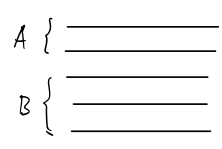
\includegraphics[scale=0.5]{chapters/res/density-operator-subsystems.png}
\end{figure}

Let the quantum system be described by a density operator $\rho^{AB}$. \\
Define the \underline{reduced density operator} for system $A$ by 

\begin{equation}
    \rho^A = tr_B [\rho^{AB}]
\end{equation}

and analogously

\begin{equation}
    \rho^B = tr_A [\rho^{AB}]
\end{equation}

Examples:
\begin{itemize}
    \item For any quantum states $\ket{a_1}, \ket{a_2} \in A$ and $\ket{a_1}, \ket{a_2} \in A$:
    \begin{equation}
        tr_B [\ket{a_1} \bra{a_2} \otimes \ket{b_1}\bra{b_2}] =
        \ket{a_1}\bra{a_2} \cdot tr[\ket{b_1}\bra{b_2}] = 
        \ket{a_1}\bra{a_2} \cdot \underbrace{\observable{b_2 | b_1}}_{\in \mathbb{C}}
    \end{equation}

    \item Given a density matrix $\rho$ for a subsystem $A$ and $\sigma$ for subsystem $B$.
    Suppose that the overall density matrix is 
    \begin{equation}
        \rho^{AB} = \rho \cdot \sigma
    \end{equation}
    Then 
    \begin{align}
        tr_B[\rho \cdot \sigma] &= \rho tr[\sigma] = \rho \\ 
        tr_A[\rho \cdot \sigma] &= \sigma tr[\rho] = \sigma 
    \end{align}

    \item $\rho^{AB} = \statepsi \bra{\psi}$ with $\psi = \frac{1}{\sqrt{2}} (\ket{00} + \ket{11})$. 
    Expanding $\rho^{AB}$ leads to

    \begin{align*}
        \rho^{AB} &= \frac{1}{\sqrt{2}} (\ket{00} + \ket{11}) (\bra{00} + \bra{11}) \\
        &= \frac{1}{2} (\ket{00}\bra{00} + \ket{00}\bra{11} + \ket{11}\bra{00} + \ket{11}\bra{11}) \\
    \end{align*}

    \begin{align*}
        \rho^A &= tr_B{\rho^{AB}} = ... = \frac{I}{2}
    \end{align*}

    Note: Composite System is in the "pure state" $\statepsi$, whereas the subsystem is described by the 
    "mixed state" $\frac{I}{2}$
    (Indeed a mixed state: $tr[(\frac{I}{2})^2] = \frac{1}{4} \cdot tr[I] = \frac{1}{2} < 1$)
\end{itemize}

Motivation / justification for partial trace:
Let $M$ be any observable on subsystem $A$, then we want that $\rho^A$ yield the same statistics
measuring $M$ as $\rho^{AB}$ for measuring $M \otimes I$. In particular

\begin{equation}
    \observable{M} = tr[M \cdot \rho^A] = tr[(M \otimes I) \rho^{AB}] = \observable{M \otimes I}
\end{equation}

for all density operators $\rho^{AB}$. The partial trace operation for computing 
$\rho^A$ from $\rho^{AB}$ is the unique operation with this property.